\section{Metodología.}
\label{sec:metodologia}

\subsection{Tecnologías empleadas.}

En el panorama actual del desarrollo móvil, los desarrolladores se enfrentan a una decisión fundamental entre el desarrollo nativo y multiplataforma. Con el crecimiento exponencial del mercado de aplicaciones móviles y la demanda de experiencias de usuario cada vez más sofisticadas, la elección tecnológica se convierte en un factor determinante para el adecuado desarrollo del proyecto. Así pues, se realizó una evaluación de las tecnologías disponibles, considerando las necesidades específicas y las tendencias actuales de la industria.


\subsubsection{Desarrollo nativo vs. multiplataforma.}

Se optó por el desarrollo nativo de la aplicación ya que ofrece mejor rendimiento, fácil acceso a todos los recursos del smartphone y está enfocado a un sistema operativo en particular (Android). Los frameworks multiplataforma actuales también ofrecen buen rendimiento e integración con las herramientas de desarrollo de Android, pero son más propensos a tener menor rendimiento, usar más recursos del sistema y generar fallos debido a las diferencias entre iOS y Android.

Esta decisión se fundamenta en la naturaleza específica del launcher, que requiere integración profunda con el sistema operativo Android para gestionar aplicaciones, controlar tiempos de uso y proporcionar una experiencia de usuario fluida y responsiva. Los resultados la comparativa se consignaron en la Tabla \ref{tab:comparacion_nativo_multiplataforma}.

\begin{table}[ht]
\centering
\caption{Comparación entre desarrollo nativo y multiplataforma para Android}
\label{tab:comparacion_nativo_multiplataforma}
\begin{tabular}{|p{0.25\textwidth}|p{0.35\textwidth}|p{0.35\textwidth}|}
\hline
\textbf{Aspecto}{\cellcolor[gray]{0.9}} & \textbf{Desarrollo Nativo Android}{\cellcolor[gray]{0.9}} & \textbf{Desarrollo Multiplataforma}{\cellcolor[gray]{0.9}} \\
\hline
Lenguaje de programación & Kotlin o Java & JavaScript (React Native), Dart (Flutter), C\# (Xamarin) \\
\hline
Rendimiento & Óptimo, optimizado específicamente para Android & Bueno, pero generalmente inferior debido a la capa de abstracción \\
\hline
Acceso a funcionalidades & Acceso total a todas las APIs y hardware específicos & Acceso limitado, requiere plugins para funcionalidades específicas \\
\hline
Experiencia de usuario & Adaptación completa a Material Design & Puede no seguir completamente las directrices de Android \\
\hline
Tiempo de desarrollo & Puede ser más largo debido a codificación específica & Más corto, código compartido entre plataformas \\
\hline
Costos de desarrollo & Más altos para Android únicamente, pero justificados & Más bajos si se desarrolla para múltiples plataformas \\
\hline
Mantenimiento & Simplificado, enfoque exclusivo en Android & Más complejo para compatibilidad específica \\
\hline
Actualizaciones de SO & Implementación inmediata con nuevas versiones & Depende de actualizaciones del framework \\
\hline
Reutilización de código & Nula entre plataformas, alta en proyectos Android & Alta reutilización multiplataforma \\
\hline
Compatibilidad & Total, diseño específico para Android & Buena, pero con posibles inconsistencias \\
\hline
\end{tabular}
\end{table}

\subsubsection{Versión objetivo de la API de Android.}

La elección de Android 10 (API 29) como versión mínima para el desarrollo de Dino Launcher se fundamenta en la convergencia entre las funcionalidades que introduce esta versión del sistema operativo, los requisitos específicos del launcher desarrollado y la posibilidad de que pueda ser ejecutado en dispositivos no tan recientes de manera satisfactoria. En la figura \ref{fig:versiones_android}, los datos de distribución de Android 10 alcanzan el 81.2\% de los dispositivos en el mercado, lo que garantiza una amplia compatibilidad con los dispositivos de los usuarios objetivo. 

\begin{figure}[ht]
\caption{Distribución de versiones de Android a nivel mundial. \cite{AndroidStudio}}
\label{fig:versiones_android}
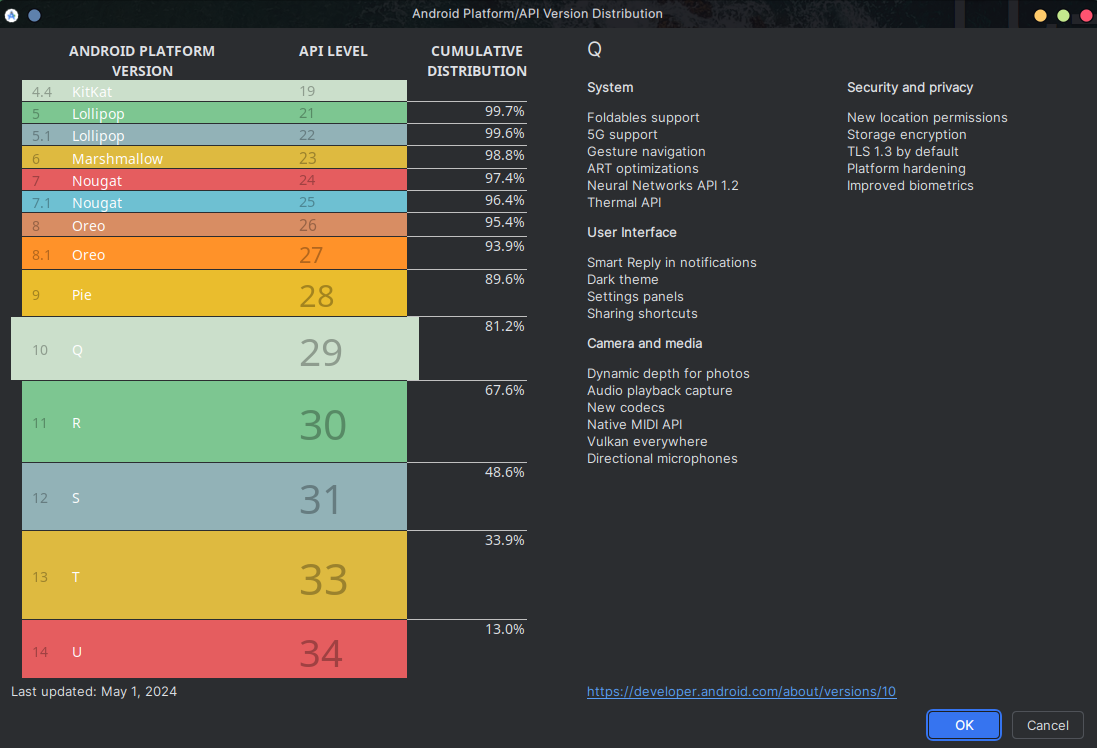
\includegraphics[width=\textwidth]{Figuras/versiones_android.png}
\centering
\end{figure}

Esta versión introduce características esenciales que hacen posible una de las funcionalidades centrales del launcher, la introducción nativa del \textbf{modo oscuro}. Esta permite al launcher mostrar automáticamente los modos claro y oscuro dependiendo de la configuración del tema del sistema, reduciendo significativamente la fatiga visual durante el uso del launcher y mejorando la experiencia de usuario, especialmente durante las horas nocturnas cuando el control del tiempo de pantalla es más crítico. 

\subsubsection{Selección del lenguaje: Kotlin.}

Las dos alternativas principales para el desarrollo nativo en Android son Java y Kotlin. Aunque Java es el lenguaje tradicional para el desarrollo Android, ha perdido terreno gracias a Kotlin y sus mejoras significativas con respecto a Java para el desarrollo móvil, principalmente en cuanto a sintaxis y características modernas. Según la encuesta anual de desarrolladores de Stack Overflow de mayo de 2024 \cite{Stackoverflow2024}, los desarrolladores que trabajan con Kotlin se sienten más cómodos con el lenguaje, al contrario de lo que se observa en Java, donde varios de los encuestados preferirían trabajar con Kotlin. La selección de Kotlin se fundamenta en los siguientes aspectos:

\begin{itemize}
    \item Google, propietario de Android, recomienda Kotlin para cualquier proyecto nuevo de Android y declaró que construiría sus herramientas de desarrollo con un enfoque Kotlin-first desde la conferencia Google I/O en 2019 \cite{Google2019}.
    \item Es un lenguaje más fácil de entender por su sintaxis simplificada y la reducción de código repetitivo (\textit{boilerplate}), reduciendo el tiempo de aprendizaje.
    \item Es un lenguaje activamente desarrollado y adaptado a las necesidades actuales de la industria.
    \item Tiene una gran comunidad y cantidad de recursos disponibles.
    \item Ofrece características modernas como corrutinas, funciones de extensión y clases de datos que facilitan el desarrollo de aplicaciones complejas.
\end{itemize}

La Tabla \ref{tab:comparacion_kotlin_java} resume las principales diferencias entre Kotlin y Java, destacando las ventajas de Kotlin para el desarrollo del launcher.

\begin{table}[ht]
\centering
\caption{Comparación entre Kotlin y Java para desarrollo Android}
\label{tab:comparacion_kotlin_java}
\begin{tabular}{|p{0.25\textwidth}|p{0.35\textwidth}|p{0.35\textwidth}|}
\hline
\textbf{Aspecto}{\cellcolor[gray]{0.9}} & \textbf{Kotlin}{\cellcolor[gray]{0.9}} & \textbf{Java}{\cellcolor[gray]{0.9}} \\
\hline
Año de lanzamiento & 2011 & 1995 \\
\hline
Sintaxis & Concisa, moderna y más legible & Extensa, más detallada y tradicional \\
\hline
Interoperabilidad & Totalmente interoperable con Java & No es nativamente interoperable con Kotlin \\
\hline
Seguridad de tipos nulos & Evita NullPointerExceptions & NullPointerExceptions son comunes \\
\hline
Compatibilidad Android & Totalmente compatible, lenguaje oficial & Compatible pero no recomendado oficialmente \\
\hline
Características modernas & Lambdas, corrutinas, extension functions, data classes & Introducción más lenta de características modernas \\
\hline
Curva de aprendizaje & Relativamente fácil para desarrolladores Java & Relativamente fácil pero más verboso \\
\hline
Productividad & Alta, gracias a sintaxis concisa & Moderada, requiere más código para tareas similares \\
\hline
Soporte y comunidad & Creciente, especialmente en Android & Muy grande y establecida, décadas de documentación \\
\hline
Desempeño & Similar a Java, optimizaciones específicas & Similar a Kotlin, rendimiento comparable \\
\hline
Ecosistema de herramientas & Totalmente soportado en Android Studio & Amplio soporte en diversas IDEs \\
\hline
\end{tabular}
\end{table}

\subsubsection{Librería de UI: Jetpack Compose.}

Jetpack Compose es el toolkit de UI más reciente y recomendado por Google para el desarrollo de interfaces en Android desde 2021, marcando un cambio paradigmático hacia la programación declarativa. Compose permite construir interfaces de usuario de manera más intuitiva, eficiente y mantenible en comparación con el sistema tradicional basado en vistas XML. Su adopción se ha consolidado como el estándar para nuevos proyectos Android, facilitando la creación de experiencias visuales modernas y adaptables.

El aspecto más relevante de Jetpack Compose es su integración nativa con Kotlin, lo que permite aprovechar plenamente las características modernas del lenguaje como las funciones lambda, la programación funcional y la sintaxis concisa, mejorando la legibilidad y mantenibilidad del código y reduciendo la cantidad de código necesario para construir interfaces. En la Figura \ref{fig:compose_vs_xml}, se muestra un ejemplo de código en Jetpack Compose que ilustra su simplicidad y claridad en comparación con el enfoque tradicional de XML para construir una interfaz que muestre las palabras \textit{"Good"} \textit{"Morning"} una arriba de la otra.

\begin{figure}[H]
\caption{Ejemplo de código en Jetpack Compose}
\label{fig:compose_vs_xml}
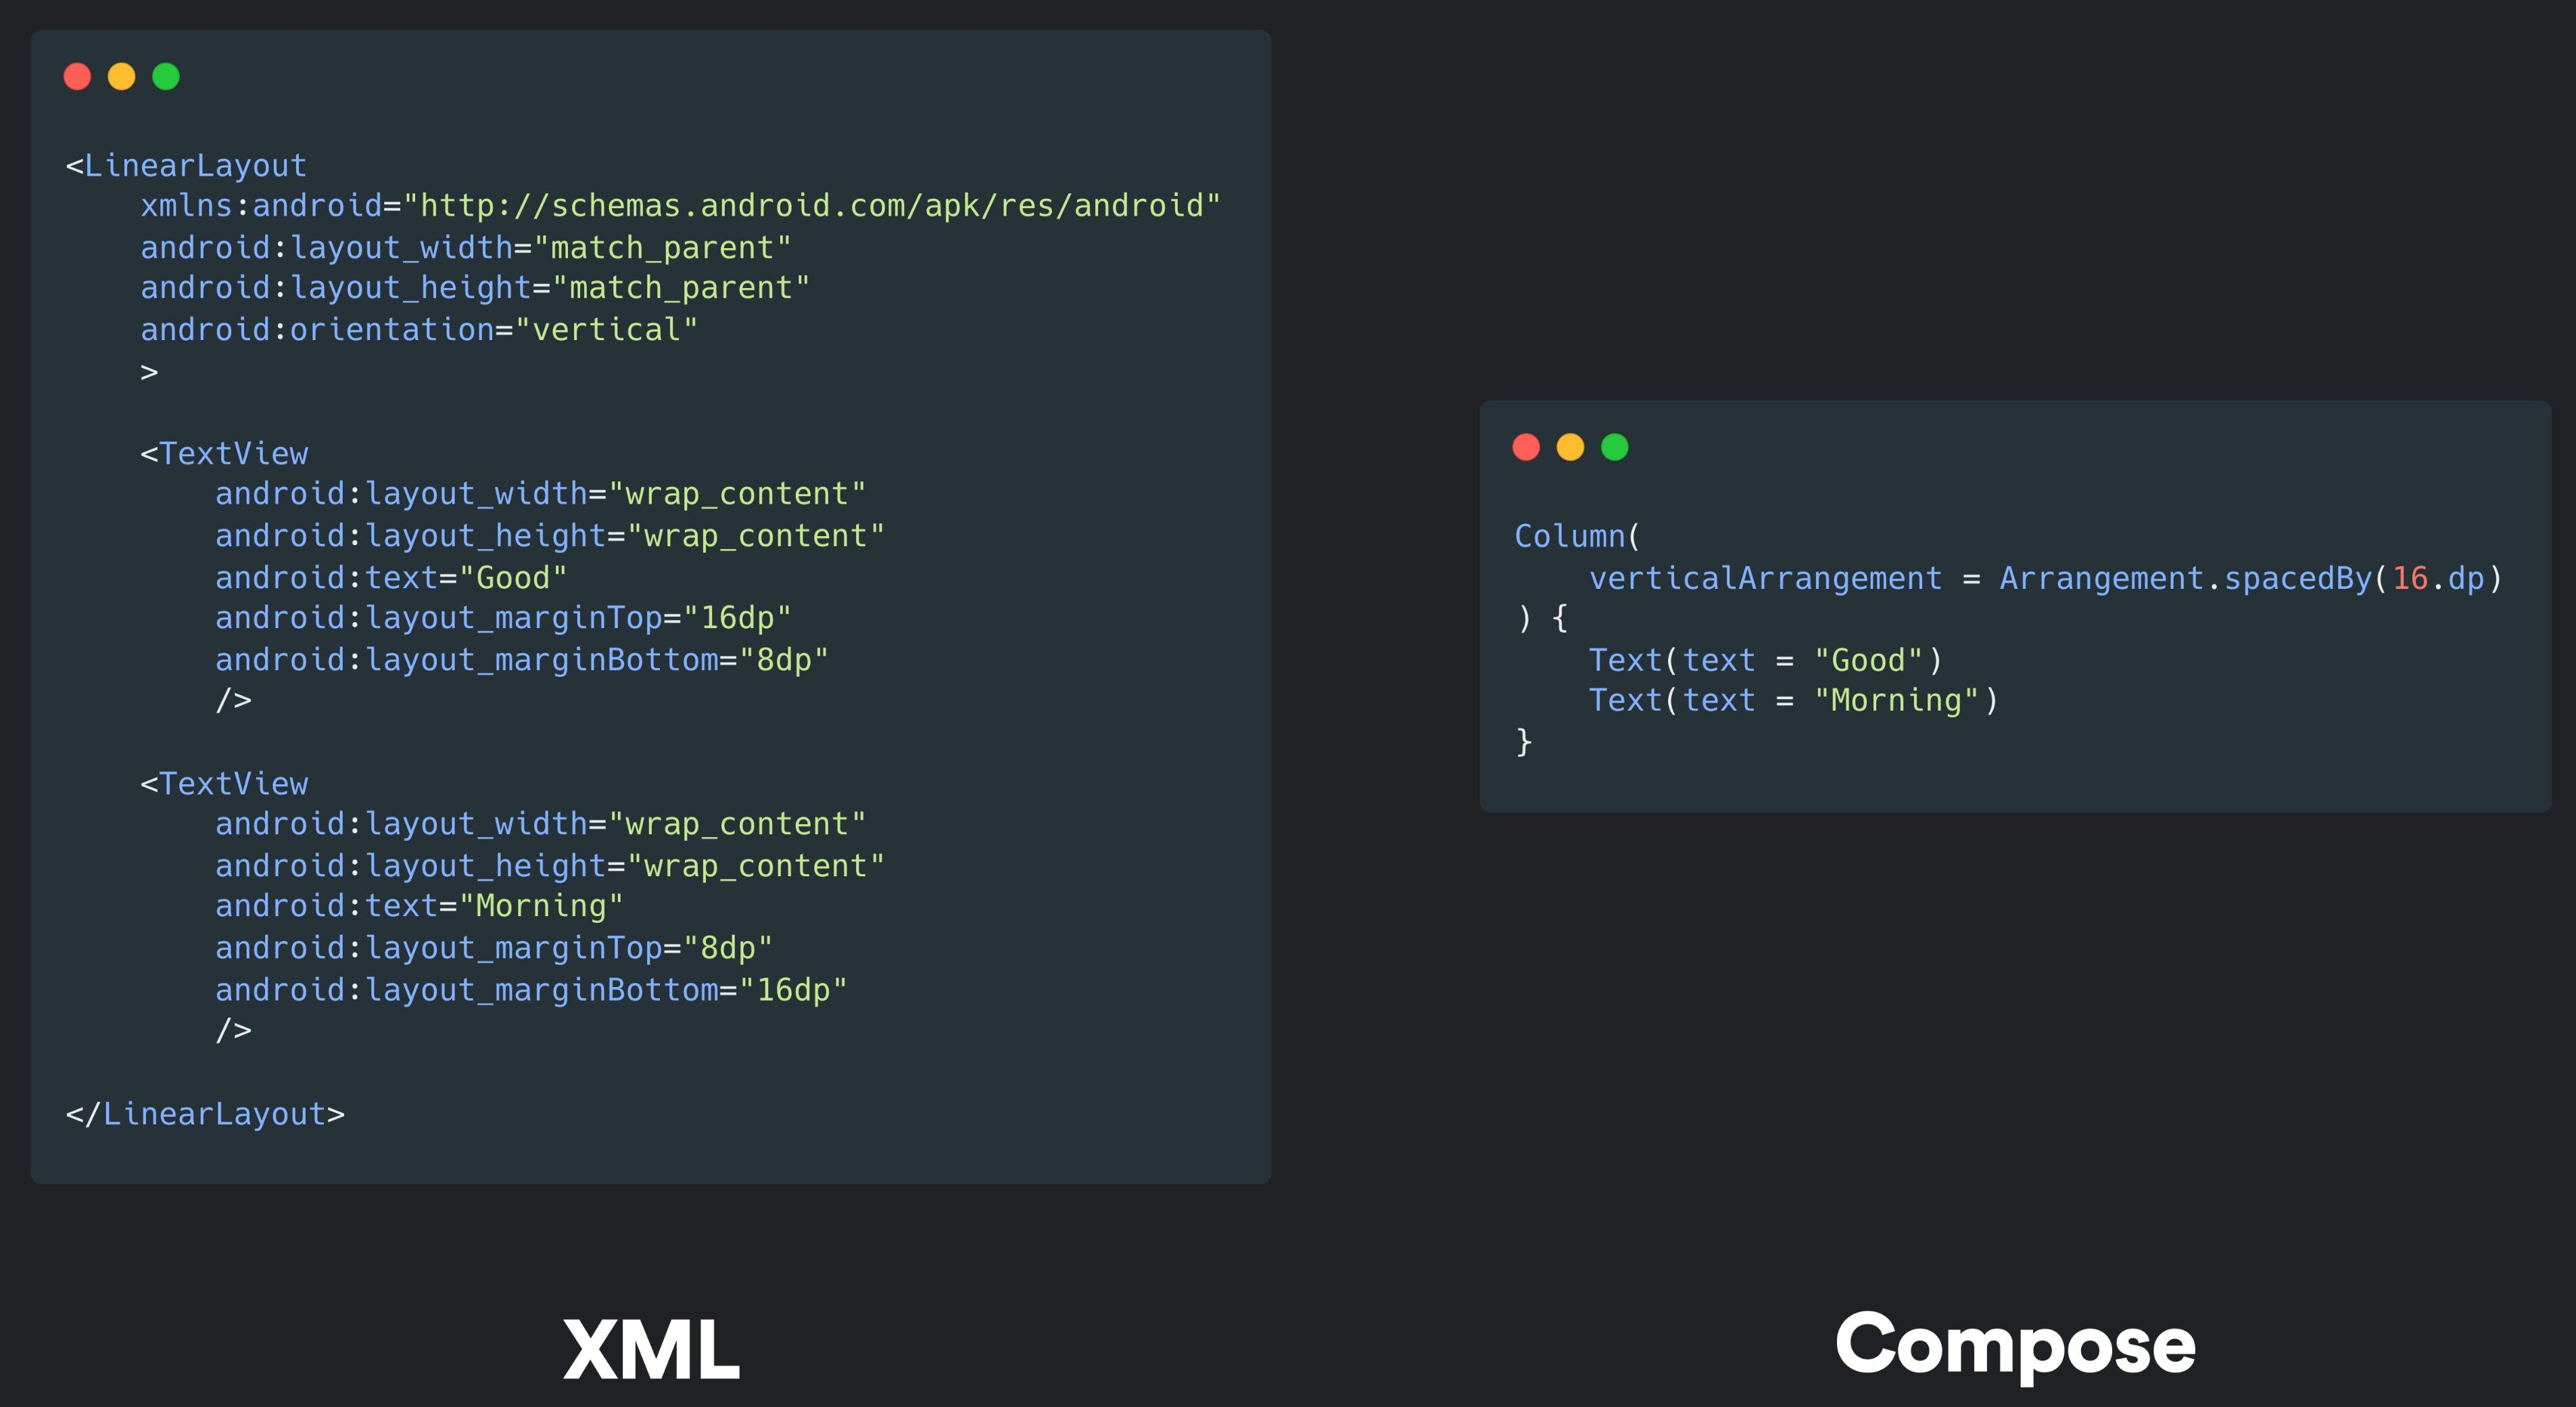
\includegraphics[width=0.88\textwidth]{Figuras/compose_vs_xml.jpg}
\centering
\end{figure}

\pagebreak

La Tabla \ref{tab:comparacion_compose_xml} presenta una comparación detallada entre Jetpack Compose y el sistema tradicional de vistas XML, destacando las ventajas técnicas que justifican la adopción de Compose para el desarrollo del launcher.

\begin{table}[ht]
\centering
\caption{Comparación entre Jetpack Compose y vistas XML para desarrollo Android}
\label{tab:comparacion_compose_xml}
\begin{tabular}{|p{0.25\textwidth}|p{0.35\textwidth}|p{0.35\textwidth}|}
\hline
\textbf{Aspecto}{\cellcolor[gray]{0.9}} & \textbf{Jetpack Compose}{\cellcolor[gray]{0.9}} & \textbf{Vistas XML}{\cellcolor[gray]{0.9}} \\
\hline
Paradigma de programación & Declarativo, describe qué mostrar & Imperativo, describe cómo construir \\
\hline
Lenguaje & 100\% Kotlin, fuertemente tipado & XML + Kotlin/Java, tipos débiles \\
\hline
Gestión de estado & Recomposición automática con State & Actualización manual de vistas \\
\hline
Animaciones & APIs nativas integradas, declarativas & Requiere configuración compleja XML/código \\
\hline
Reutilización de código & Composición funcional, alta reutilización & Herencia de vistas, reutilización limitada \\
\hline
Curva de aprendizaje & Requiere conocimiento de programación funcional & Familiar para desarrolladores tradicionales \\
\hline
Rendimiento & Recomposición inteligente, optimizado & Inflado de layouts puede ser costoso \\
\hline
Depuración & Compose Inspector integrado & Layout Inspector tradicional \\ 
\hline
Tamaño de APK & Comparable o menor & Puede ser mayor con layouts complejos \\
\hline
Interoperabilidad & Completa con vistas XML existentes & No compatible con Compose sin wrappers \\
\hline
Soporte de temas & Material Design 3 nativo & Requiere configuración manual extensa \\
\hline
Testing & Testing declarativo con ComposeTestRule & Testing complejo de interacciones UI \\
\hline
Mantenimiento & Simplificado, lógica en un solo lugar & Complejo, lógica distribuida en XML y código \\
\hline
Adopción empresarial & Creciente, recomendado por Google & Establecido, pero en desuso gradual \\
\hline
\end{tabular}
\end{table}

\subsubsection{Persistencia de datos: Room.}

Room es una biblioteca de persistencia que forma parte de Android Jetpack \cite{Jetpack} y proporciona una capa de abstracción sobre SQLite. Está diseñada específicamente para simplificar el trabajo con bases de datos en Android, combinando la potencia de SQLite con la comodidad y seguridad de tipos del desarrollo en Kotlin \cite{Room}. Entre las principales ventajas de utilizar Room en el desarrollo Android, se encuentran la posibilidad de observar cambios en los datos de manera reactiva con LiveData y Flow, facilitando la actualización automática de la interfaz de usuario; el soporte nativo para corrutinas, que permiten la ejecución de manera asíncrona utilizando \textit{suspend functions}, evitando bloqueos en el hilo principal y el uso de anotaciones para reducir código repetitivo (como \texttt{@Entity}, \texttt{@Dao} o \texttt{@Database}) para generar automáticamente el código necesario y realizar operaciones en SQLite. En la figura \ref{fig:room}, se muestra el flujo de datos de Room entre la base de datos y la aplicación desarrollada.

\begin{figure}[ht]
\caption{Flujo de datos de Room. \cite{Room}}
\label{fig:room}
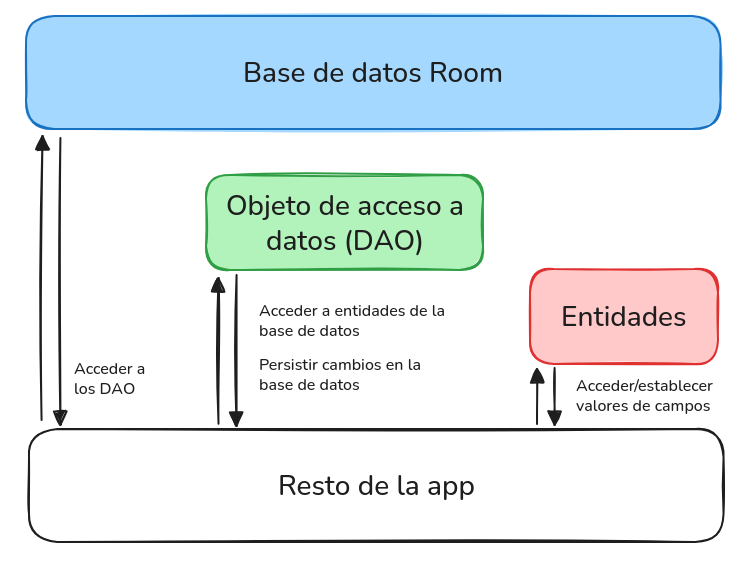
\includegraphics[width=\textwidth]{Figuras/room.png}
\centering
\end{figure}

La selección de Room como solución de persistencia de datos por encima de alternativas basadas en la nube, como Firebase, se fundamenta en las características específicas del launcher y sus requerimientos funcionales en la sección \ref{sec:requerimientos_funcionales}. El proyecto no requiere que los datos estén disponibles en múltiples dispositivos o se sincronicen en tiempo real, ya que el launcher está diseñado para funcionar de manera individual en cada dispositivo. Además, el tipo de información que maneja la aplicación no demanda características de red en tiempo real ni almacenamiento de datos complejos o de gran tamaño. La naturaleza personal y privada de estos datos hace innecesaria la implementación de sistemas de autenticación de cuentas de usuario o gestión de perfiles en la nube, simplificando la arquitectura del sistema y minimizando el uso de recursos que puedan llegar a consumir las funciones de red.
